\chapter{User Guide}
\label{ch:user_guide}

In the previous chapters, we developed and evaluated several methods for a Known-item search task. In this chapter, we provide a user guide for our implementation of the aforementioned techniques. This chapter only covers user interaction and does not cover experimenting with new datasets nor the overview of the implementation.

The user can access the application via a web-based interface. Once the webpage is opened, we can see by default a module for search based on the collage (refer to \autoref{ch:object_location}). The second module includes face similarity search (\autoref{ch:face_search}). We proceed to describe both modules.

\section{Running the Application}

The easiest way to run the application is to install Docker\footnote{\url{https://docs.docker.com/desktop/}}. Once the Docker is installed, it is enough to run following commands from the top-level directory, i.e., where \verb+README.md+ is located.

\vspace{0.5cm}

\begin{boxedverbatim}
# ./thesis-grizzly/
$ docker build . -t app
$ docker run -p 8000:8000  \
  -v $PWD/image_representations:\
      /diplomova_praca/static/image_representations \
  -t app
\end{boxedverbatim}

\vspace{0.5cm}

Once the application is running, we can access it via browser at following web address: \url{http://127.0.0.1:8000/}. The first initialization takes longer, the website will load itself once the initialization completes. 

\subsection*{Included Dataset}

The provided demo includes a small dataset of images to search on. These images come from Open Image Dataset\footnote{\url{https://opensource.google/projects/open-images-dataset}, CC-by 4.0}. The dataset contains 20\,035 images, for which we computed the region splitting for 2x4 regions. For an approach using the antepenultimate layer, we only provide extracted features for half of the dataset, due to the size limit of the attachments. Finally, we extracted 528 faces from the dataset for the search by face similarities (with the same settings as described in \autoref{ch:face_search}).

The data, which the model uses is in the directory \verb+image_representation+. In the next chapter, we describe how to work with custom data. It is possible to either replace the existing ones or to create a new directory and update the path in the provided command.

\section{Modules}

Our application is separated into two modules: spatial search and face search. Users can switch between the modules in the top right corner. Now we shortly describe a typical interaction of the user with the system for each module.

\subsection{Search by Collage}

The default module, which opens, is search by collage. On the screen, we can see a canvas for creating the queries and some control elements. On the first load, a target image (the searched scene) is displayed for several seconds over the canvas. During the creation of the collage, we can always access the target image by clicking on the image button (``Display hint''), see \autoref{fig:ui_collage}.

\subsubsection*{Creating a Collage}

We can create custom collages on the canvas. To add an image to the canvas, we can either \emph{paste} it, or add it via the URL of the image. To paste an image, it needs to be available in the clipboard. The easiest way to do that for most images is to right-click on the image and select ``Copy image''. We can also recommend a selective screenshot feature, which can speed up the copying of the images and add the possibility of selecting only a part of the image. For Windows 10, it is possible via key combination Shift + Win Key + S. Linux users with KDE may use Spectacle (usually invoked via Print Screen key) or a similar utility.

There is no limitation on the number of images in the collage, although the increased number of images may reduce the performance (as they may give misleading hints), and also it prolongs the computation time needed for the query to be processed.

Once the image is placed in the canvas, we can resize it by grabbing the bottom right corner or move it by dragging. To remove the image from the canvas, click on the \verb+x+ button in the top right corner. To submit the query, click the ``Query'' button. By default, automatic querying is turned on, i.e., after each movement or resizing, the system automatically queries the dataset. This can be turned off, which comes handy if the model with longer inference time is used.

It is possible to switch between the approaches used for feature extraction. The list of available approaches can be accessed by clicking on the three dots, next to the query button.

\subsubsection*{Displayed Results}

\begin{figure}
    % \centering
    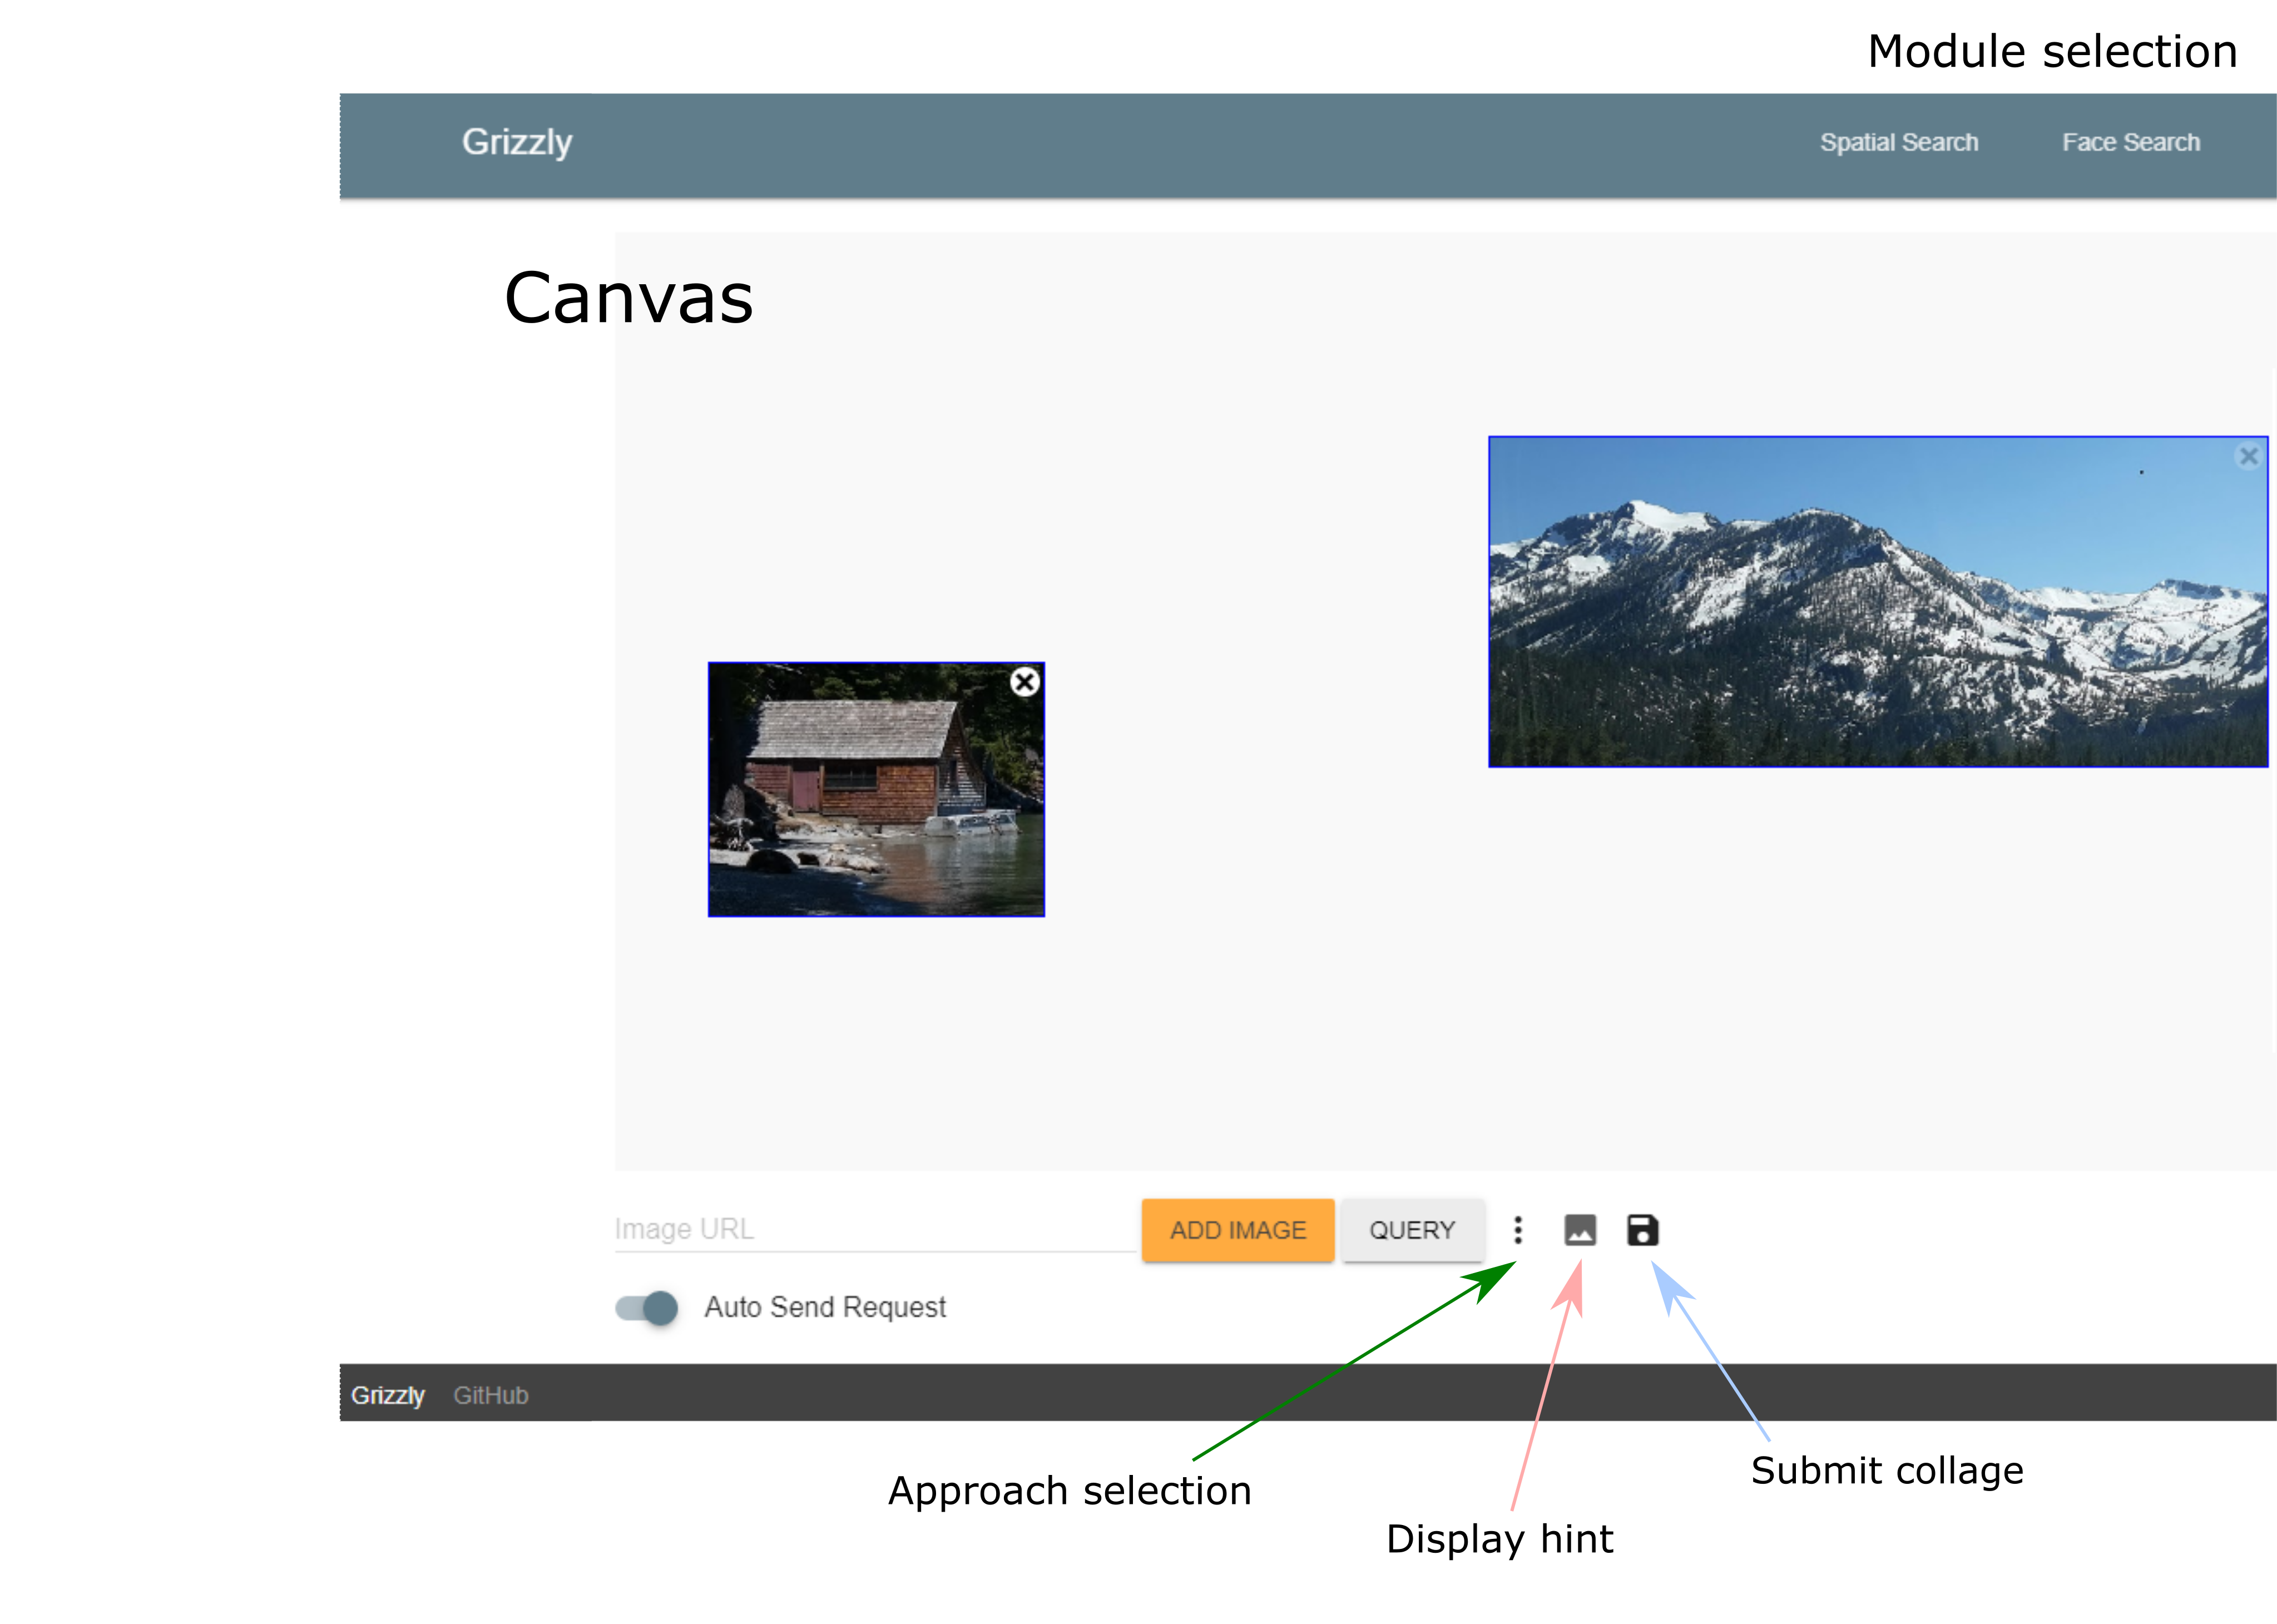
\includegraphics[width=0.9\linewidth]{img/spatial_ui.png}
    \caption{User interface for creating collages}
    \label{fig:ui_collage}
\end{figure}

By default, the application displays only the best 100 matched results. The images are reloaded after each successful query. The top of the Results section also displays the rank of the searched item. This helps the user to learn how to use the tool more effectively. The winning regions are highlighted as well for the regions' search by an orange rectangle.

Results are presented based on the ranking, as we described in \autoref{s:task_formulation}. More similar results are displayed first. If the image is not present in the loaded dataset, the rank will not be displayed. This may be a case if the features for a given approach are not available for all images in the dataset.

\subsection{Search by Face Similarity}

\begin{figure}
    \centering
    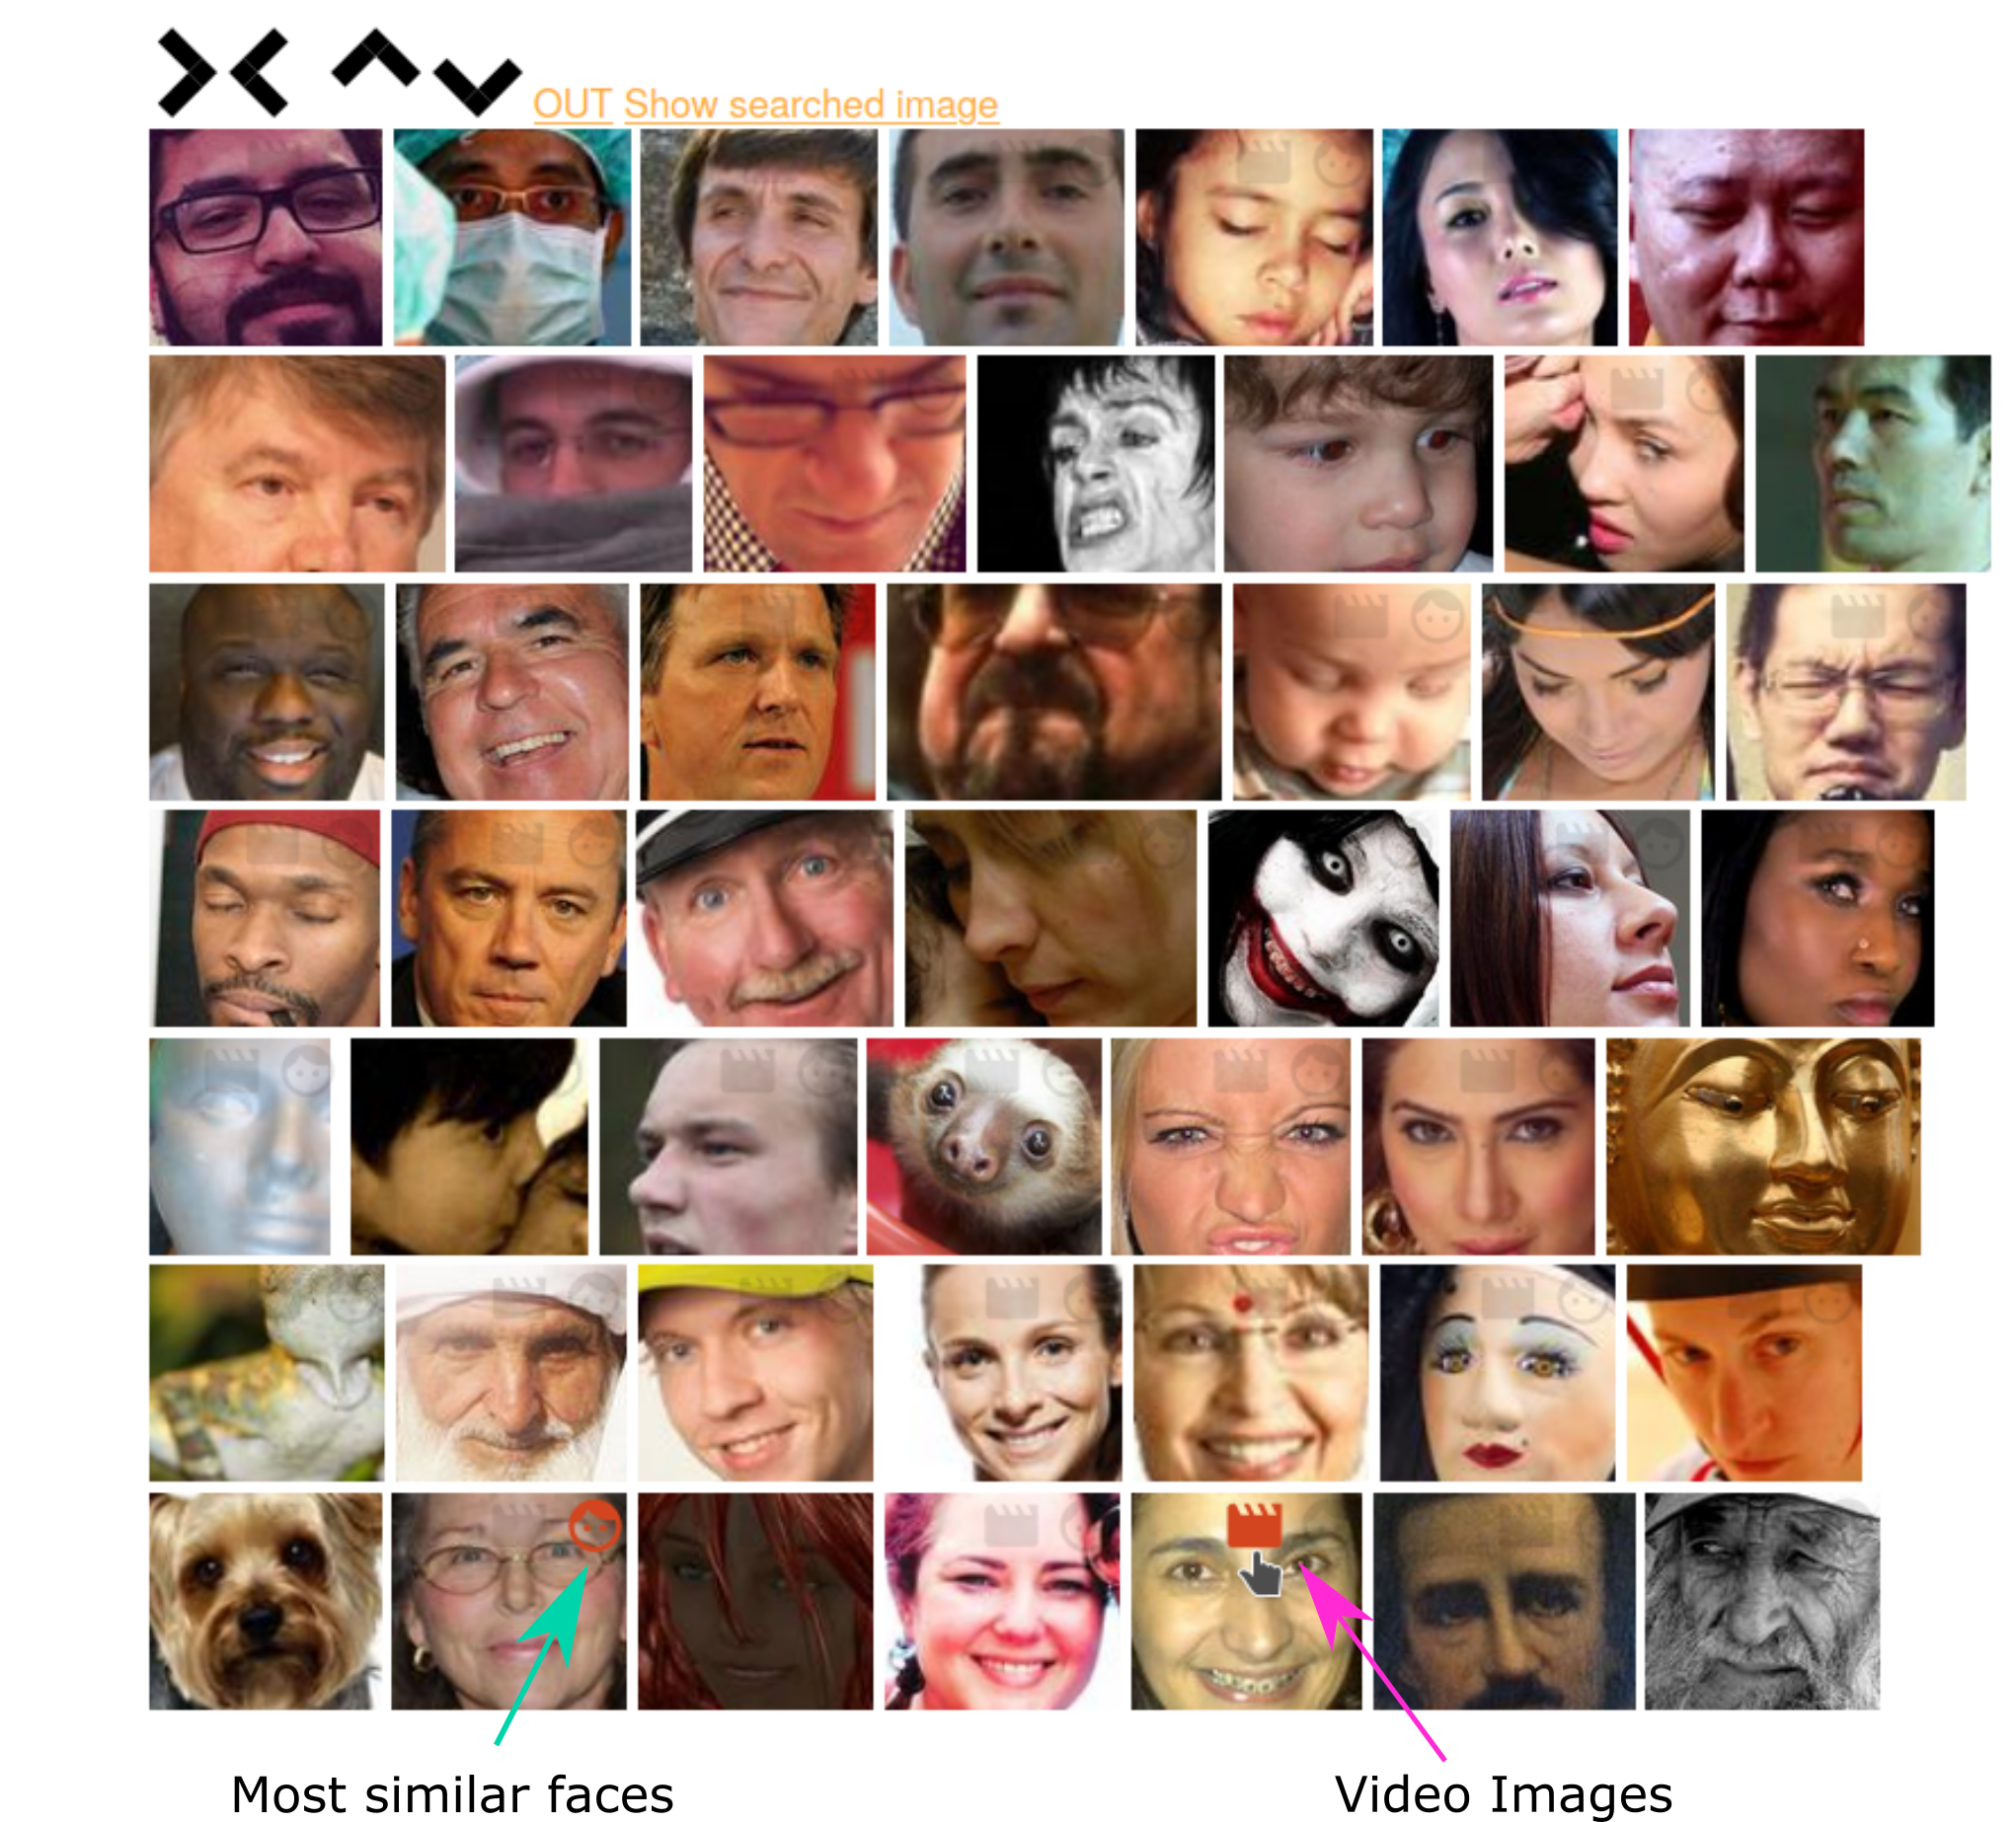
\includegraphics[width=\linewidth]{img/face_grid.png}
    \caption{Top layer of our traversal structure.}
    \label{fig:face_grid_app}
\end{figure}

Upon loading the face module, there is a grid with faces, and also a target image is displayed. Like the Search by collage module, the target image can be accessed at any moment by clicking on \verb+Show the image+. 

The grid, which is displayed, represents the top layer of the multilevel structure. This layer fully fits into a display; therefore, move commands do not have an effect. We can step up from any (except top layer, where it does not have any effect) layer by clicking on the \verb+Zoom Out+.

By clicking at any face, we step down one layer. The image which we clicked is in the center of the next layer, if possible. This is not possible for images near the corners and edges. In such case, the grid is displayed in a way that full display is used, and the clicked image is as close to the center as possible.

Each image in the traversal structure also supports two additional operations: show images from the video and show the closest faces. In the case of images, which did not come from the videos (the case of the demo dataset), the images displayed by the first option, are arbitrary. The second option displays all images, which contain a face similar to the queried one. Both these options are available by corresponding icons in the top right corner of the face, available at any layer. A top layer for our demo dataset is displayed in the \autoref{fig:face_grid_app}


\chapter{Extracting Features for a Custom Dataset}
\label{ch:custom_dataset}

In the previous chapter, we described how to run a demo with a preprocessed dataset of images. In this chapter, we describe the steps required to run the application for a new set of images. If we do not want to change the dataset but only evaluate different approaches (i.e., changing the underlying neural network), it is enough to do only the corresponding step.

Our feature extraction is a two-step process. We again use Docker, to avoid dependency problems. The extraction process belongs to separate module -- \verb+diplomova_praca_lib+. Therefore, we firstly change the working directory, and then we build a single docker container, which we use for all extractions.

\vspace{0.5cm}
\begin{boxedverbatim}
$ cd diplomova_praca_lib
$ docker build . -t lib
\end{boxedverbatim}
\vspace{0.5cm}

The user needs to prepare a directory with images to be processed. If the images come from videos, this directory should be further divided into subdirectories. Each subdirectory should then contain images from one video.

\section{Feature Extraction for Collage Approaches}

In this section, we provide an example of extracting features for our system for both collage approaches: regions and the approach using the last convolution block. In this example, we extract features by \verb+MobileNetV2+, using regions \verb+2x4+ with the \verb+input_size=96+. The system expects equally sized images.

\vspace{0.5cm}
\begin{boxedverbatim}
$ images="/path/to/images/"
$ intermediate_output="/path/to/intermediate_output/"
$ features="/path/to/features/"

$ docker run \
  -v $images:/images \
  -v $intermediate_output:/feature_records \
  lib \
   python diplomova_praca_lib/annotate_images.py \
    --images_dir=/images --save_location=/feature_records \
    --feature_model=mobilenetv2 --num_regions=2,4 \
    --input_size=96

$ docker run \
  -v $intermediate_output:/feature_records \
  -v $features:/features \
  lib \
    python diplomova_praca_lib/preprocess_data.py \
      --input=/feature_records --output=/features 
      --transform --regions --explained_ratio=128
\end{boxedverbatim}

\vspace{0.5cm}

Parameter options for feature extraction are:
\begin{itemize}
    \item \verb+--feature_model+: \verb+resnet50v2antepenultimate+, \verb+resnet50v2+, \\ \verb+mobilenetv2antepenultimate+, \verb+mobilenetv2+, 
    \item \verb+--input_size+: depends on the model used, check with Keras Applications
    \item \verb+--num_regions+: other values evaluated in this thesis were 2x3, 3x5. Other viable options are allowed.
\end{itemize}

The second step includes preprocessing with optional \acrshort{pca} dimension reduction. The parameters are:
\begin{itemize}
    \item \verb+--empty_pipeline+: no \acrshort{pca} is applied, data are only preprocessed forming structure for the application
    \item \verb+--explained_ratio+: \acrshort{pca} into given number of components is applied
    \item \verb+--regions+: to specify that the data reflect the regions' structure
\end{itemize}

The content of the \verb+$features+ directory can be then copied to the corresponding directory (see  \autoref{s:dir_structure}) and immediately used, by running the app (see \autoref{ch:user_guide}).

\section{Feature Extraction for Face Similarity}

For the extraction of faces and their encodings, we use similar steps as in the previous section:

\vspace{0.5cm}
\begin{boxedverbatim}
$ images="/path/to/images/"
$ intermediate_output="/path/to/intermediate_output/"
$ face_features="/path/to/face_features/"

$ docker run \
  -v $images:/images \
  -v $intermediate_output:/feature_records \
  lib \
   python diplomova_praca_lib/annotate_images.py \
    --images_dir=/images --save_location=/feature_records \
    --feature_model=faces

$ docker run \
  -v $intermediate_output:/feature_records \
  -v $face_features:/features \
  lib \
    python diplomova_praca_lib/preprocess_face_data.py \
      --input=/feature_records --output=/features \
      --crop_size=0.08
\end{boxedverbatim}
\vspace{0.5cm}

where the \verb+crop_size+ specifies filtering criteria on the minimum area covered by the face in the image.

\subsection{Training Self-organizing Map}

After obtaining the face encodings, we can train the underlying Self-organizing Map, which we use to obtain a grid of faces for the bottom layer.


\vspace{0.5cm}
\begin{boxedverbatim}
$ face_features="/path/to/face_features/"
$ trained_som="/path/to/trained_som/"

$ docker run \
  -v $face_features:/features \
  -v $trained_som:/output \
  lib \
   python diplomova_praca_lib/train_som.py \
    --input=/features \
    --iterations=200000
\end{boxedverbatim}
\vspace{0.5cm}

For \verb+train_som.py+ additional arguments as \verb+learning_rate+, \verb+sigma+, \verb+distance+ may be explored. The scripts saves all intermediate Self-organizing Maps and also plots the errors during the training. It is possible to choose any of the stored \acrshort{som}s for the application and observe the differences between them.

\section{Running the Server with Custom Data}
\label{s:dir_structure}

We can replace any of the existing data by the new ones, either in their original location \verb+image_representations+, or we can create a new location for the data with following structure:


\vspace{0.5cm}
\begin{boxedverbatim}
image_representations/
    faces/
        features/
            faces.npz
        som/
            som.pickle
    images/
        000/
            image1.jpg
        001/
            image2.jpg
    regions/
        model-mobilenetv2,dir=000.npz
        model-mobilenetv2,dir=001.npz
    spatial/
        model-mobilenetv2antepenultimate,dir=000.npz
        model-mobilenetv2antepenultimate,dir=001.npz
\end{boxedverbatim}
\vspace{0.5cm}

It is not necessary to provide all the data for all the approaches. Only the modules with correctly provided data will work as expected.
